
\iffalse \bibliography{../bibliography.bib} \fi

\chapter{Results}


\section{Voxels}

The size of voxel chunks affects rendering performance and the cost of modification.
Since modifying the terrain requires the entire chunk mesh to be reconstructed, it is ideal to have smaller chunks.
However, larger chunk sizes reduce the number of draw calls.
Figure \ref{fig:voxel_plot_1} shows the relationship between chunk size and render performance for a fixed view distance.
Since the same amount of geometry is rendered for each chunk size tested, the decrease in performance at low chunk size can be attributed to draw calls and other engine overhead.
Figure \ref{fig:voxel_plot_2} shows the modification cost for each chunk size.
These results indicate that that a chunk size of 32 or 64 is a good compromise between render performance and modification cost.

\begin{figure}
	\centering
\begin{tikzpicture}
	\begin{axis}[
		xlabel=Chunk Size (ft),
		ylabel=Frame Time (ms),
		width=11cm
		]
		\addplot[color=green,mark=*] coordinates
		{
			(4,649.37)
			(8,163.43)
			(16,40.69)
			(32,9.04)
			(64,2.27)
			(128,2.16)
			(256,1.85)
		};
	\end{axis}
\end{tikzpicture}
	\caption{
		Voxel terrain rendering performance for different chunk sizes.
		For each chunk size, view distance is set to 512 feet.
	}
	\label{fig:voxel_plot_1}
\end{figure}

\begin{figure}
	\centering
\begin{tikzpicture}
	\begin{axis}[
		xlabel=Chunk Size (ft),
		ylabel=Modification Time (s),
		width=11cm
		]
		\addplot[color=green,mark=*] coordinates
		{
			(4,0.0002)
			(8,0.0010)
			(16,0.0068)
			(32,0.0342)
			(64,0.301)
			(128,2.42)
			(256,24.44)
		};
	\end{axis}
\end{tikzpicture}
	\caption{
		Graph of modification cost (i.e. digging) for different chunk sizes.
	}
	\label{fig:voxel_plot_2}
\end{figure}

\section{Clipmaps}

One motivation for using geometry clipmaps is an even distribution of screen space to polygon.
\editor{need figure of polygonal screen-space density compared to a simple grid}

Another advantage of geometry clipmaps is the exponential relationship between layer count and view distance.
Figure \ref{fig:clipmaps_plot_1} and \ref{fig:clipmaps_plot_2} show the relationship between clipmap layers, view distance, and frame time in milliseconds for a scene containing only the clipmaps terrain and a skybox.

\begin{figure}
	\centering
\begin{tikzpicture}
	\begin{axis}[
		xlabel=Layer Count,
		ylabel=Frame Time (ms),
		width=11cm
		]
		\addplot[color=red,mark=*] coordinates
		{
			(1,0.245)
			(2,0.27)
			(3,0.28)
			(4,0.288)
			(5,0.305)
			(6,0.321)
			(7,0.342)
			(8,0.351)
			(9,0.37)
			(10,0.389)
			(11,0.412)
			(12,0.435)
			(13,0.442)
			(14,0.447)
			(15,0.453)
			(16,0.463)
			(17,0.476)
			(18,0.485)
		};
	\end{axis}
\end{tikzpicture}
	\caption{
		Geometry clipmaps render time for a given number of clipmap layers.
	}
	\label{fig:clipmaps_plot_1}
\end{figure}

\begin{figure}
	\centering
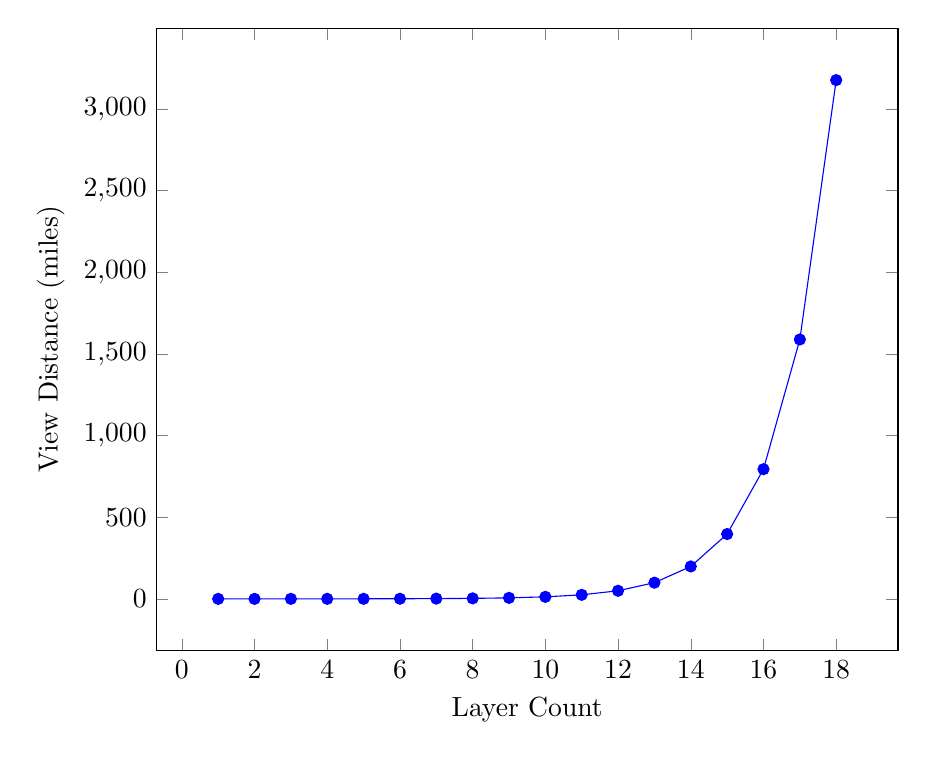
\begin{tikzpicture}
	\begin{axis}[
		xlabel=Layer Count,
		ylabel=View Distance (miles),
		width=11cm
		]
		\addplot[color=blue,mark=*] coordinates
		{
			(1,0.024242424)
			(2,0.048484848)
			(3,0.096969697)
			(4,0.193939394)
			(5,0.387878788)
			(6,0.775757576)
			(7,1.551515152)
			(8,3.103030303)
			(9,6.206060606)
			(10,12.41212121)
			(11,24.82424242)
			(12,49.64848485)
			(13,99.2969697)
			(14,198.5939394)
			(15,397.1878788)
			(16,794.3757576)
			(17,1588.751515)
			(18,3177.50303)
		};
	\end{axis}
\end{tikzpicture}
	\caption{
		Geometry clipmaps view distance and for a given number of clipmap layers.
	}
	\label{fig:clipmaps_plot_2}
\end{figure}

There is a linear relationship between frame time and layer count, but an exponential relationship between view distance and layer count.
For a relatively minor increase in frame time an absurd view distance of over 3000 miles can be achieved.
For reference, the largest possible view distance on earth is around 300 miles, between two mountains in South America. \cite{viewdistancemaxearth}

Larger individual layer sizes increase view distance and reduce polygon screen-space at the cost of performance.
\editor{Graph of performance over size of layers}

The addition of a geometry shader normal calculation simplifies the terrain generation process and improves visual quality, but incurs a small performance hit.
\editor{Geometry shader normal calculation performance hit}


\section{Vegetation}

The far layers of the vegetation system are rough visual approximations of the closeup tree meshes, but are significantly less costly for rendering.
\editor{Graph of performance meshes vs. impostors vs. batched simple geometry}

Increasing the size of tree groups decreases CPU performance while improving rendering performance.
\editor{Graph of chunk size performance}


\section{Water}


\section{Depth Buffer Precision}

Our system supports very large view distances.
Setting the far plane at sufficient distance for our scene significantly degrades the performance of the depth buffer, even with 32 bits of precision.

The problem is that the depth buffer stores reciprocal depths, such that most of the depth buffer is alloted for nearby fragments.
To improve depth buffer performance for far distances, we use the inverted depth buffer trick.
By using a DirectX compatibility feature of OpenGL, we can use a depth buffer ranging from zero to one instead of negative one to one.
Then, by storing depths reversed from the conventional direction, we can utilize the inherent distribution of floating point precision to even out the distribution of depth values in our scene.
The conventional depth direction has near values at zero and far values at one.
However, floating point precision is higher for values closer to zero.
By storing near depths at one and far depths at zero, the additional floating point precision creates a pseudo-logarithmic distribution of depth values.

This results in a significant reduction in depth fighting artifacts.
See figure \editor{comparison of reverse depth turned off and on}.

